\section{Durchführung}

Die Messungen werden mit Hilfe eines Ultraschallechoskop, einer Ultraschallsonde und einem Computer durchgeführt. Mithilfe des Computer können die Piks der Spannung in Abhänigikeit der 
Zeit aufgezeichnet werden. Das verwendete Verfahren ist das Impuls-Echo-Verfahren.

\subsection{Acrylblock}
Zunächst wir ein Acrylblock mit unterscheidlichen Bohrungen auf unterschiedlichen Höhen untersucht. Dazu wird dieser zunächst mittels einer Schiebelehre ausgemessen, inklusive der Höhe und
dicke der Bohrungen im Block. \\
Es wird ein Kontaktmittel zwischen dem Block und der Sonde verwendet, da die Luft ein sehr guter Absorber ist. Der Acrylblock ist in \autoref{fig:acrylblock} dargestellt.
\begin{figure}
    \centering
    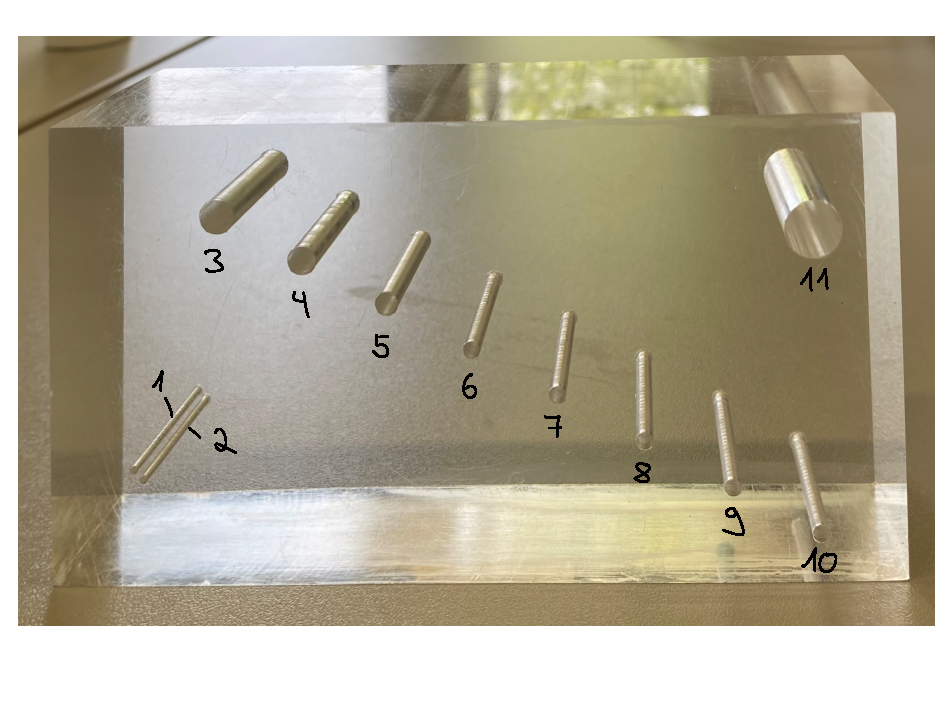
\includegraphics[width=11cm]{US1quader.pdf}
    \caption{Acrylblock.}
    \label{fig:schall}
  \end{figure}


\subsection{Auge}
Es wird ebenfalls ein Phantomauge mit der Ultraschallsonde untersucht. Ebenfalls wie zuvor wird Kontaktgel verwendet. Das Bild welches am Computer generiert wir, wird gespeichert und 
die Peaks in \autoref{sec:Auswertung} ausgewertet.



